\documentclass{beamer}
\newcommand{\myfont}{\rmfamily\normalsize\upshape\mdseries}
\newcommand{\degree}{^\circ}
\newcommand{\R}{\mathbb{R}}
\newcommand{\F}{\mathbb{F}}
\title{\sffamily Final Big RC}
\subtitle{\textbf{Exercises}\\ }
\institute[UM-SJTU JI]{University of Michigan-Shanghai Jiao Tong University Joint Institute}
\author{Kulu}
\usepackage{graphicx}
\usepackage{picinpar}
\usepackage{indentfirst}
\usepackage{chemformula}
\usepackage{geometry}
\usepackage{subfigure}
\usepackage{appendix}
\usepackage{amsfonts,amsmath,amssymb}
\usepackage{enumerate}
\usepackage{float}
\usepackage{geometry}
\usepackage{latexsym}
\usepackage{listings}
\usepackage{multicol,multirow,multido}
\usepackage{tabularx}
\usepackage{ulem}
\usepackage{tikz}
\usepackage{xcolor}
\usepackage{cite}
\usepackage{setspace}
\usepackage{textpos}
\usepackage{booktabs}
\usepackage{mathtools, nccmath}
\usepackage{hyperref}
\usetheme[dove]{Boadilla}
\usecolortheme{dolphin}
\useoutertheme{miniframes}

\begin{document}
\usebackgroundtemplate{\tikz\node[opacity=0.05]{
        \centerline{
\includegraphics[
                height=\paperheight]{kulu.jpg}}
    };}
\begin{titlepage}
    \begin{center}
        VV186 - Honors Mathmatics II
    \end{center}
\end{titlepage}
\myfont

\begin{frame}
    \begin{figure}[htbp]
        \centering
        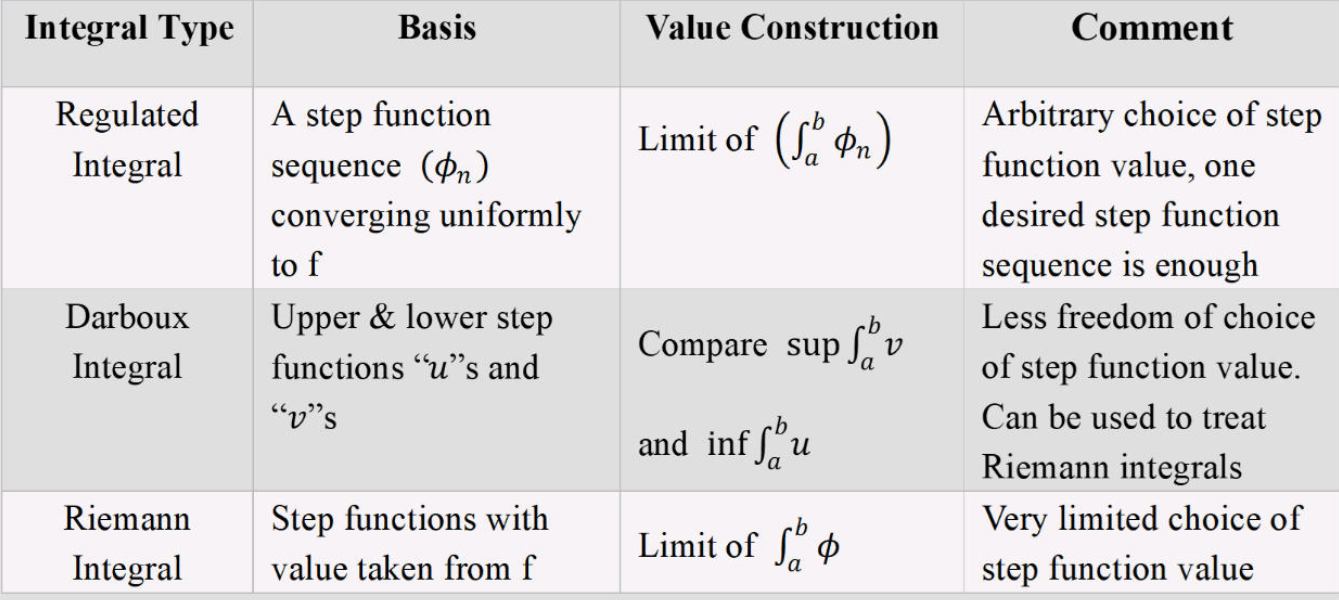
\includegraphics[width=12cm]{integral.png}
    \end{figure}
\end{frame}

\begin{frame}
    \frametitle{Regulated $\&$ Step Function \textcolor{red}{Exam Problem (last year)}}
    Let f:[a,b]$\to \mathbb{R}$, f is monotonic on [a,b], prove that f is regulated.

\end{frame}

\begin{frame}
    \frametitle{Symmetry}
    1. $\int_{0}^{+\infty}\frac{\ln x}{1+x^2} dx$

    2. $\int_{0}^{\frac{\pi}{2}}\ln (\sin x) dx$

    3. $\int_{0}^{\pi} x \ln (\sin x) dx$
\end{frame}

\begin{frame}
    \frametitle{Improper Integral ———— Useful Conclusions}
    f is defined on $[a,+\infty]$ (a>0), K>0, then

    (1) if $0\leq f~(x) \leq \frac{K}{x^p}$ for $x\in [a,+\infty)$, and $p>1$, then  $\int_{a}^{+\infty}f~(x) dx$ converges.

    (2) if $f~(x) \geq \frac{K}{x^p}$ for $x\in [a,+\infty)$, and $p\leq 1$, then  $\int_{a}^{+\infty}f~(x) dx$ diverges.
\end{frame}

\begin{frame}
    \frametitle{Improper Integral}
    1. Is $\int_{1}^{+\infty}\frac{\sin(x)}{x^p} dx (p>1)$ convergent or divergent ?

    2. Is $\int_{0}^{+\infty}[(1-\frac{\sin x}{x})^{-\frac{1}{3}}-1] dx$ convergent? Is it absolutely convergent?
\end{frame}

\begin{frame}
    \frametitle{Taylor Series}
    Let $f~(x)=\ln (1+x)$.

    (1) Find the Taylor Series of f.

    (2) Find its radius of convergence.

    (3) Find points of which the series converge, and prove it.
\end{frame}

\begin{frame}
    \frametitle{Reference}
    \begin{itemize}
        \item 2021-VV186 Final Big RC Exercises.
    \end{itemize}
\end{frame}
\begin{frame}
    \frametitle{The End}
    This is our last RC! Thanks for all the support and companion throughout the all semester! We are very glad to be your VV186 Taa!

    Maybe you are sill indulged in integration and Taylor expansions, but here comes a full stop for VV186.

    VV186 is the first stop to manifest the beauty and rigidity of college mathematics. You've been formally accepted to such vast universe of mathematics, roaming about those rigid logics and mind-blowing proofs. You will learn more theories and applications in the future, and here is the start.

    Wish you all best grades. Believe us, no matter what the final grade is, your efforts will never tell lies. The true happiness hides itself in the comprehension and reflection along the journey.

    Wish you good luck, wish you a lifetime keen on math.
    You are always welcome to contact us! Bye.

\end{frame}
\end{document}